\documentclass[12pt]{article}
\usepackage{array}
\usepackage{listings}
\usepackage{graphicx}
\usepackage{color}
\usepackage{hyperref}
\usepackage{caption}
\usepackage[%
    left=2.50cm,%
    right=2.50cm,%
    top=2.50cm,%
    bottom=2.50cm%
]{geometry}%

\lstset{
  basicstyle=\fontfamily{lmvtt}\selectfont\small,
  columns=fullflexible,
}
\title{Rapport de la semaine du 11 avril 2022}
\author{TUELEAU Tom}
\begin{document}
\maketitle
\section{Introduction}
Ce document a pour objectif de faire l'état d'avancement du stage. Celui-ci résumera donc le travail effectué la semaine du 11 avril 2022.
Je vous présente dans un premier temps mon installation et comment j'ai aménagé mon espace de travail. Dans une deuxième partie,
nous verrons le travail que j'ai effectué sur les capteurs et le microcontrôleur lors des 5 jours. Enfin, une dernière partie introduira le travail 
que je prévois d'effectuer lors des semaines à venir. 

\section{Installation}
Lors de cette semaine, j'ai pu m'installer au niveau du rucher. J'y ai apporté du matériel emprunté à l'IUT (oscilloscope, shield ethernet pour
arduino Uno) et du matériel personnel (arduino, capteurs, câbles ...). Nous avons aussi à disposition un switch relié à la fibre. J'ai été, et je serai,
de nouveau amené à me déplacer à Béziers afin de récupérer du matériel et pour manipuler des systèmes électroniques.

\begin{center}	
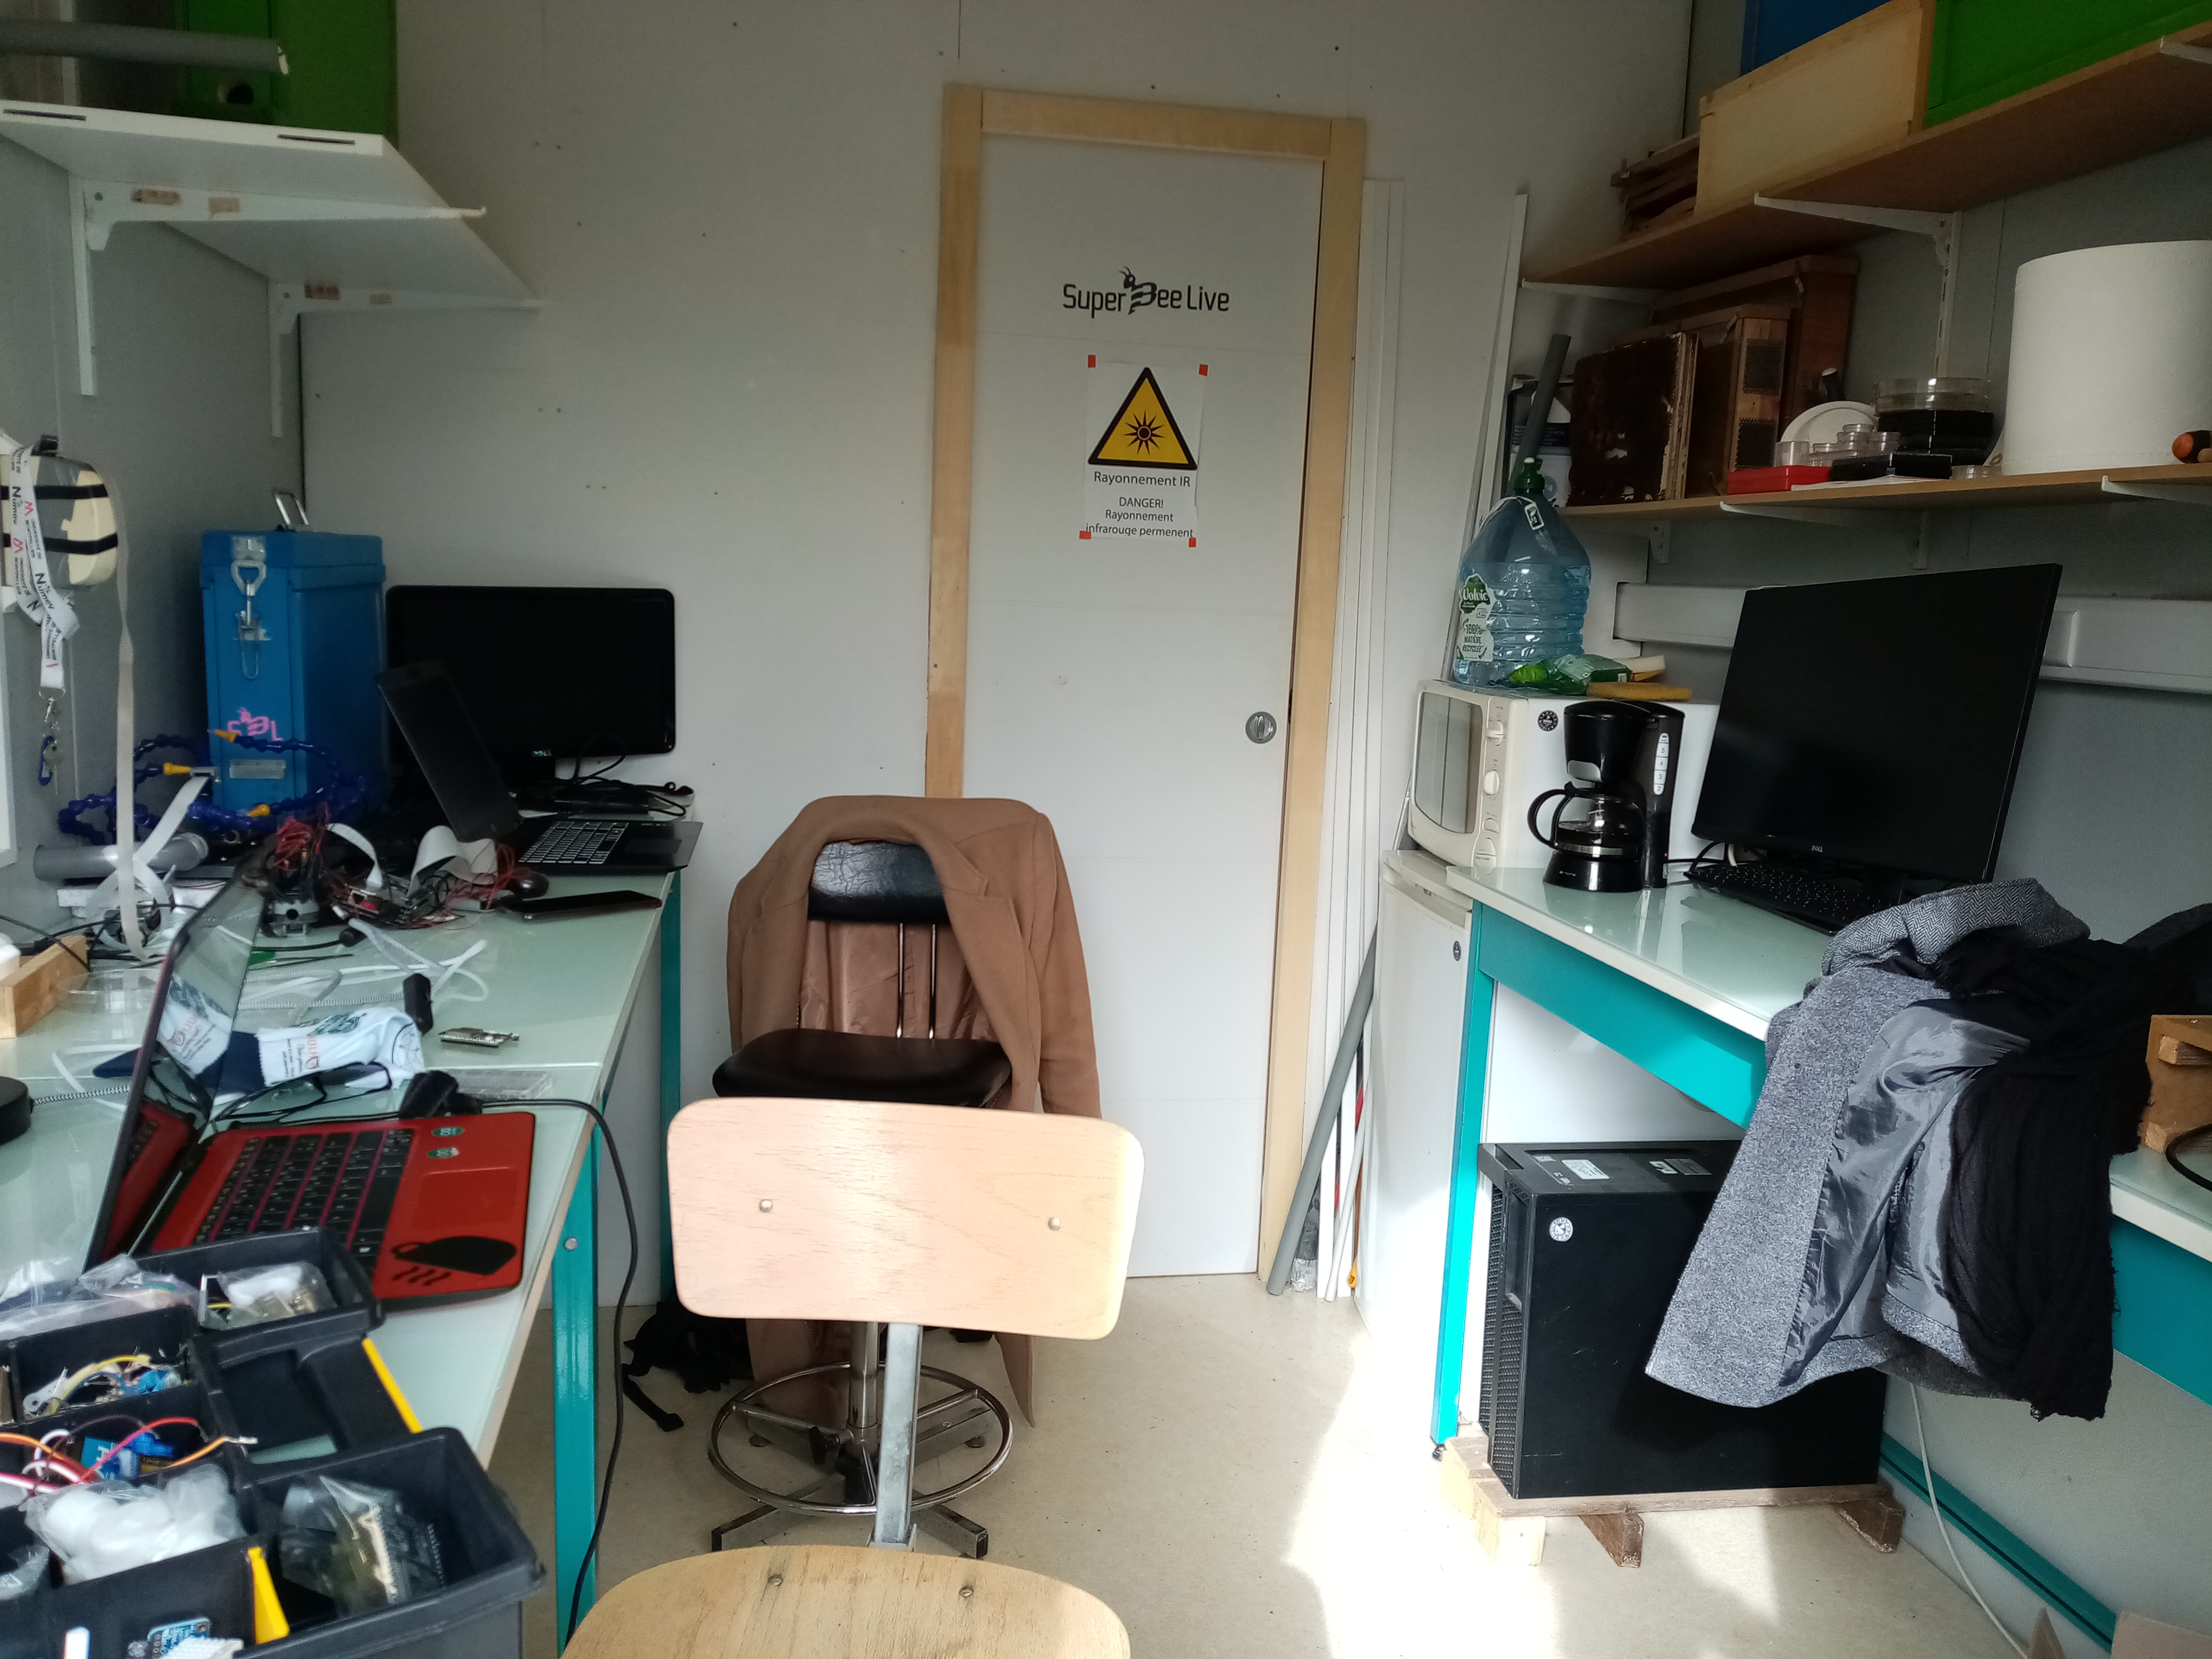
\includegraphics[scale=0.075]{interieur_rucher.jpg}
\captionof{figure}{Intérieur du rucher}
\label{image1}
\includegraphics[scale=0.075]{exterieur_rucher.jpg}
\captionof{figure}{Extérieur du rucher}
\label{image2}
\end{center}

\section{Choix des composants}

\subsection{Mise en contexte}

Le but de cette section est d'énoncer les possibilités que j'ai trouvées en ce qui concerne les composants liés à la première partie du stage. 
Ceux-ci pourront changer tout au long de la mission. L'objectif de cette première partie est le suivant :\\ (Extrait ordre de mission)\\ 
\\
Nous avons besoin de mettre en place une première installation avec un micro-controleur et
des capteurs dans la ruche afin de faire un "proof of concept" simple pour pouvoir afficher les
données enregistrée sur le site internet où les vidéos des abeilles seront diffusées.\\
\\
Les données à enregistrer seront :\\
— Température\\
— Hygrométrie\\
— Capteur de vibration fixé sur une gaufre de la ruche\\
\\
Elles devront être remontées en MQTT sur un serveur déjà mis en place.
Le tout doit être opérationnel (fonctionnel et dans la ruche) avant le 15 Mai 2022.
\\
\\
Je dois donc concevoir un prototype rapidement afin de répondre aux besoins énoncés ci-dessus.
Dans cette partie, je vous présente les choix faits lors de la première semaine, nous commencerons par voir les différentes
possibilités pour le micro-contrôleur. Ensuite, j'évoquerais les modèles des capteurs d'hygrométrie et de température aux quels j'ai songé.
Enfin, je reviendrais sur le cas du capteur de vibration .

\subsection{Choix des composants}

\subsubsection{Micro-controleur}
Le micro controleur doit pouvoir :\\
\\
	- Récolter les données des differents capteurs\\
	- Envoyer les données via MQTT\\
	- Mise en place rapide et facile\\
	\\
De ces trois critères, j'ai trouvé deux solutions possibles. 
Tout d'abord un arduino muni d'un shield Ethernet pourrait nous permettre dans un premier temps d'avoir un système 
connecté à internet et simple à mettre en place.
Dans un second temps, j'ai pensé à un Esp32 qui permettrait de faire transiter les données en Wifi et qui est plus petit. 
Étant familiarisé avec les deux solutions je n'ai pas de préférence. J'ai cependant commencé à travailler sur l'arduino, car j'avais
le matériel à disposition.

\subsubsection{Capteur de température et d'hygrométrie }
Pour répondre à ce besoin, j'ai opté pour un Si7021. J'ai fait ce choix, car le capteur était directement à disposition et que je l'avais déjà programmé. Leurs caractéristiques sont les suivantes :\\
\\
Température :\\
\begin{center}
    \begin{tabular}{|l|l|}
	\hline
	    Plage de valeur & Résolution \\
	\hline
	    -40C - 125C & 0,4C \\
	\hline
    \end{tabular}
\end{center}
Humidité:\\
\begin{center}
    \begin{tabular}{|l|l|}
	\hline
	    Plage de valeur & Résolution \\
	\hline
	    0\% - 80\% & 0,3\% \\
	\hline
    \end{tabular}
\end{center}

\subsubsection{Capteur de vibration}
Le capteur de vibration est la partie que je connais le moins du projet. J'ai pu trouvé deux solutions.\\
 Une première à l'aide d'un capteur piézo-électrique et une seconde avec un  microphone. Ces deux capteurs étant les seules possibilités que j'avais à ma disposition, 
 j'ai décidé de les tester afin de savoir si elles pouvaient répondre aux besoins du projet.\\
\\
 Les deux références sont :\\
- p37e pour le piézo-électrique\\
- INMP441 pour le microphone.\\

\section{Travail effectué}
\subsection{Capteur Piézo-Electrique}

Afin d'analyser les caractéristiques du capteur, j'ai commencé par chercher des documents en rapport avec celui-ci. Les recherches n'ayant pas 
été très concluantes, je suis très vite passé à l'analyse du capteur. J'ai commencé par relier la sortie de celui-ci à un oscilloscope, ensuite je le fixe
sur la table avec du scotch, puis, j'effectue des coups plus ou moins forts à une distance constante de celui-ci. J'ai donc pu relever des tensions allant de 20mV à 680mV.
Étant donné que nous cherchons à étudier les mouvements des abeilles, il me semble plus logique de me baser sur les valeurs les plus petites. Celles-ci correspondant à un frottement de stylo.
Par la suite j'ai donc cherché comment effectuer une amplification du signal. Je suis très rapidement tombé sur des montages à amplificateur opérationnel (AOP). J'ai donc commencé
à les étudier et ai pu expérimenter plusieurs montages notamment un montage amplifieur non-inverseur dont vous pouvez voir les clichés ci-dessous.

\begin{center}	
	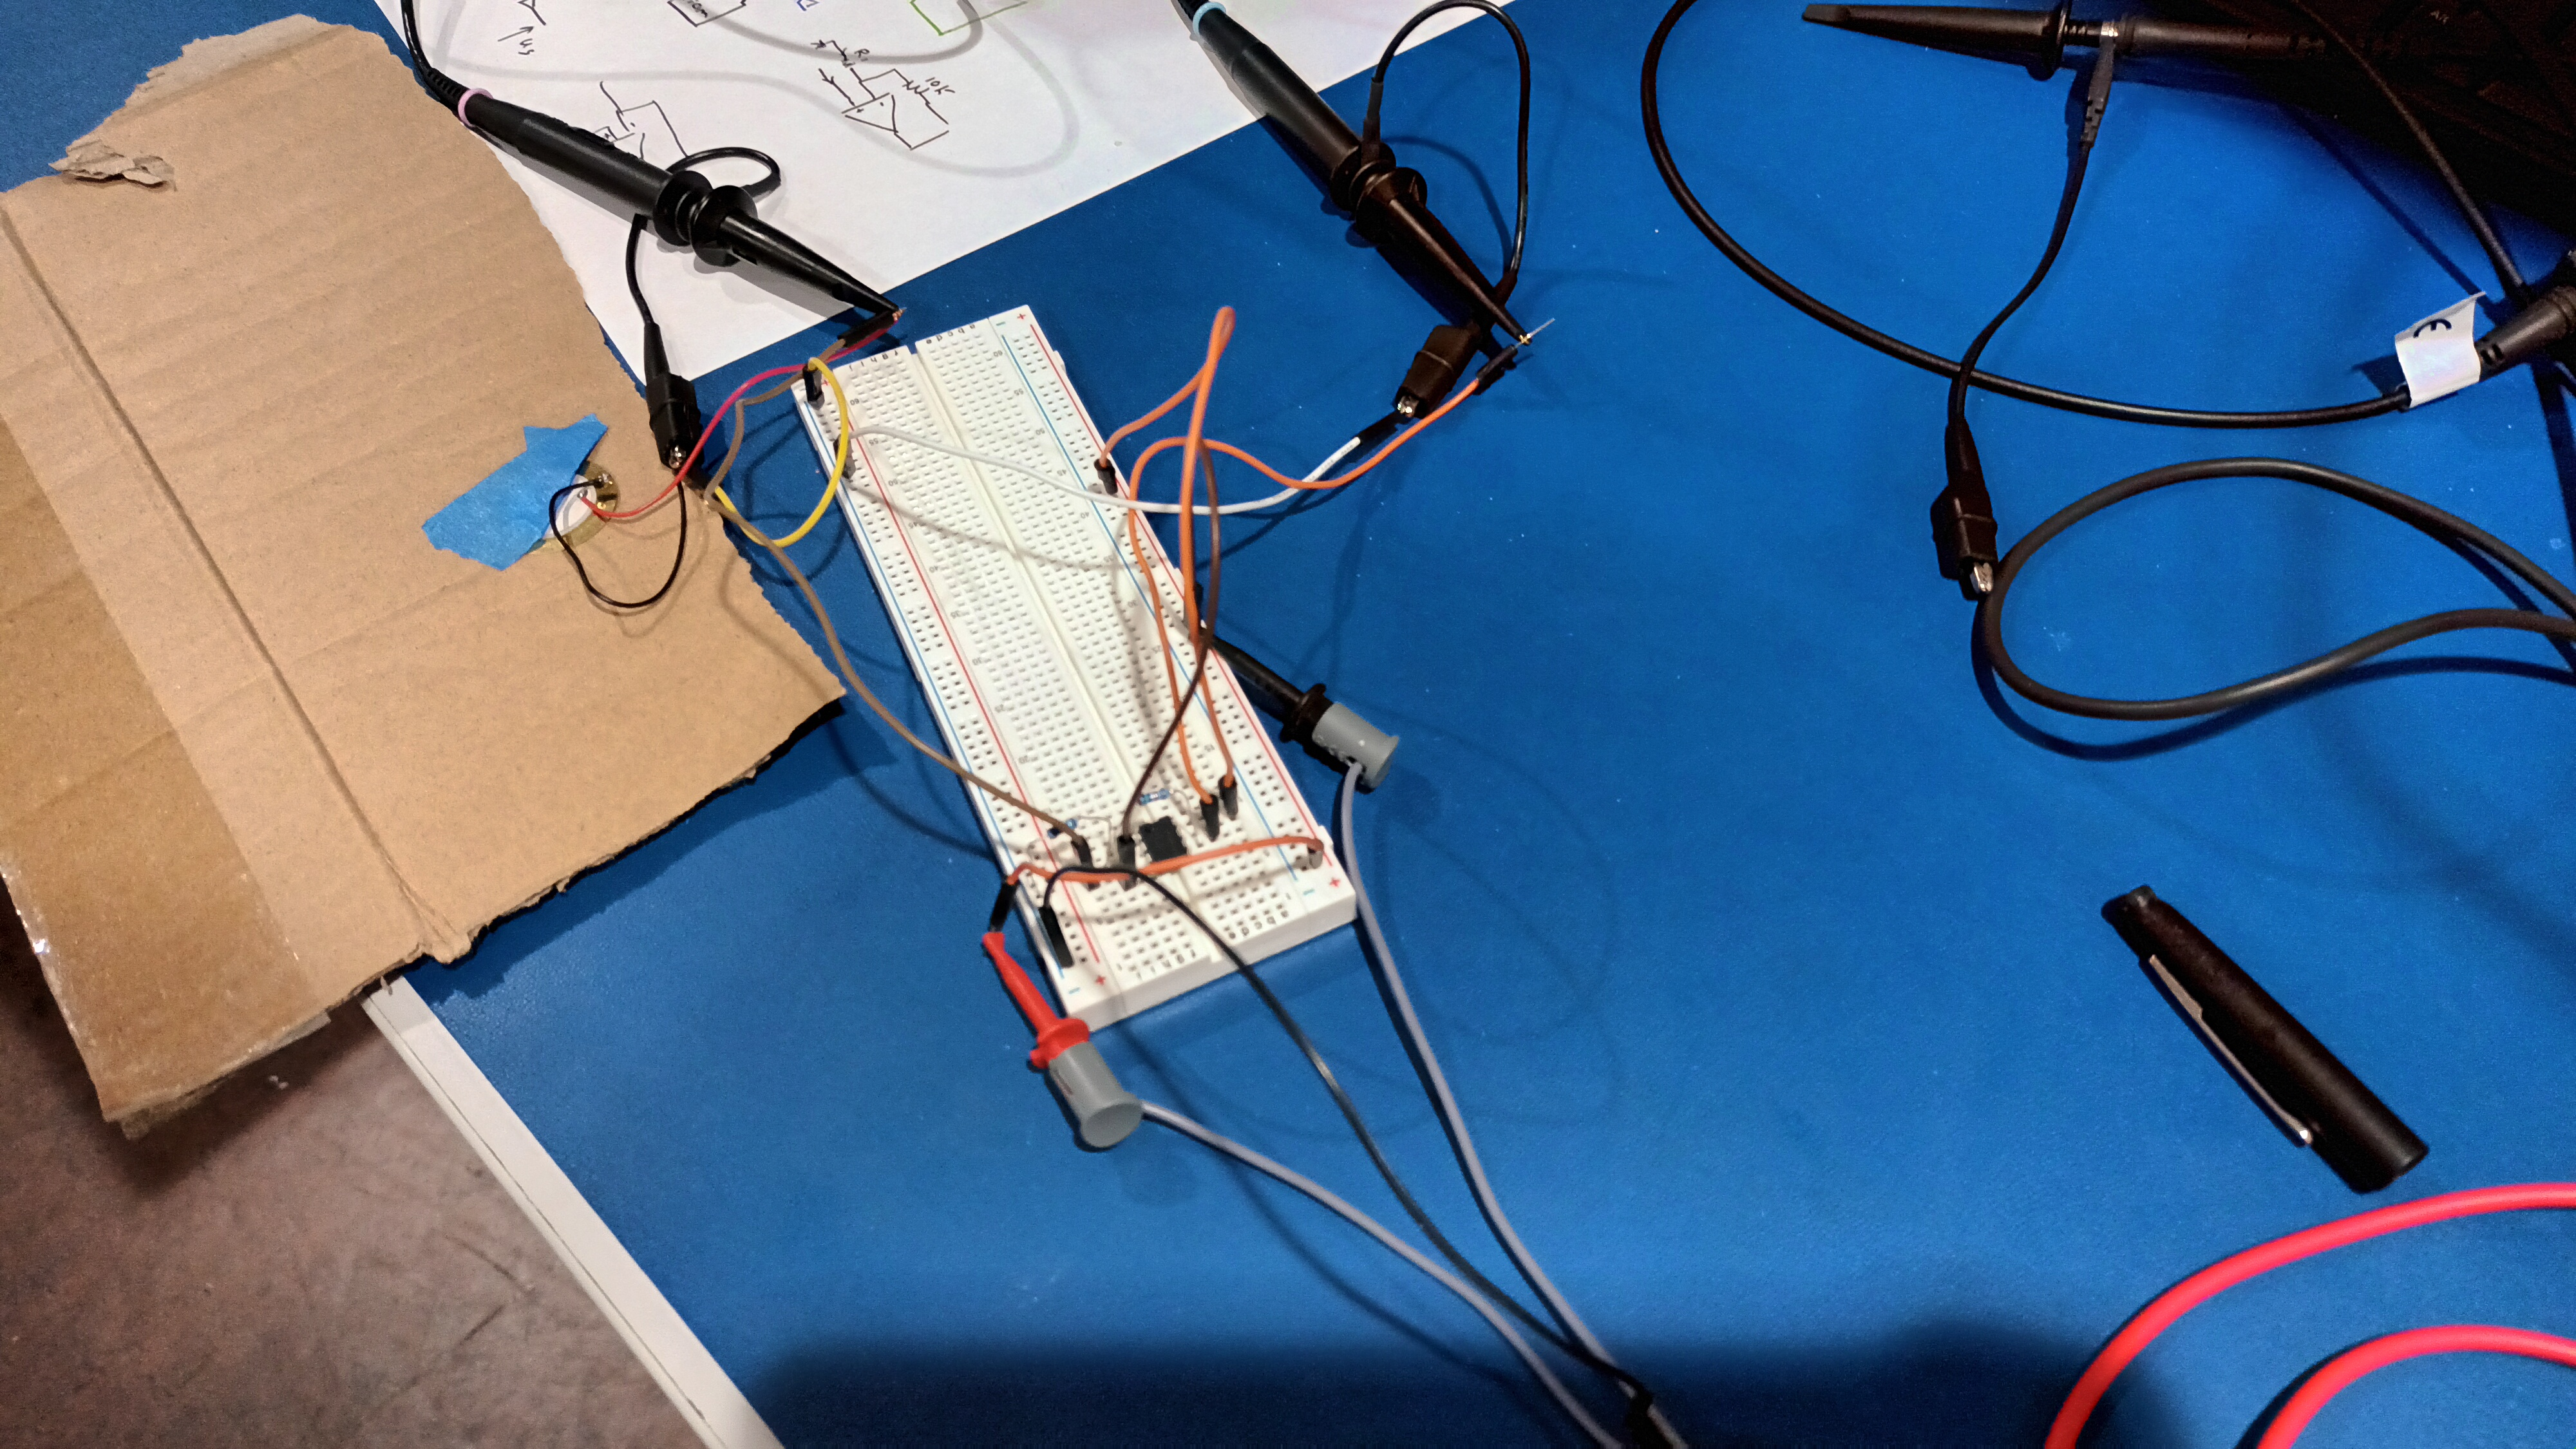
\includegraphics[scale=0.08]{montage_piezo_aop.jpg}
	\captionof{figure}{Montage piezo AOP }
	\label{image3}
	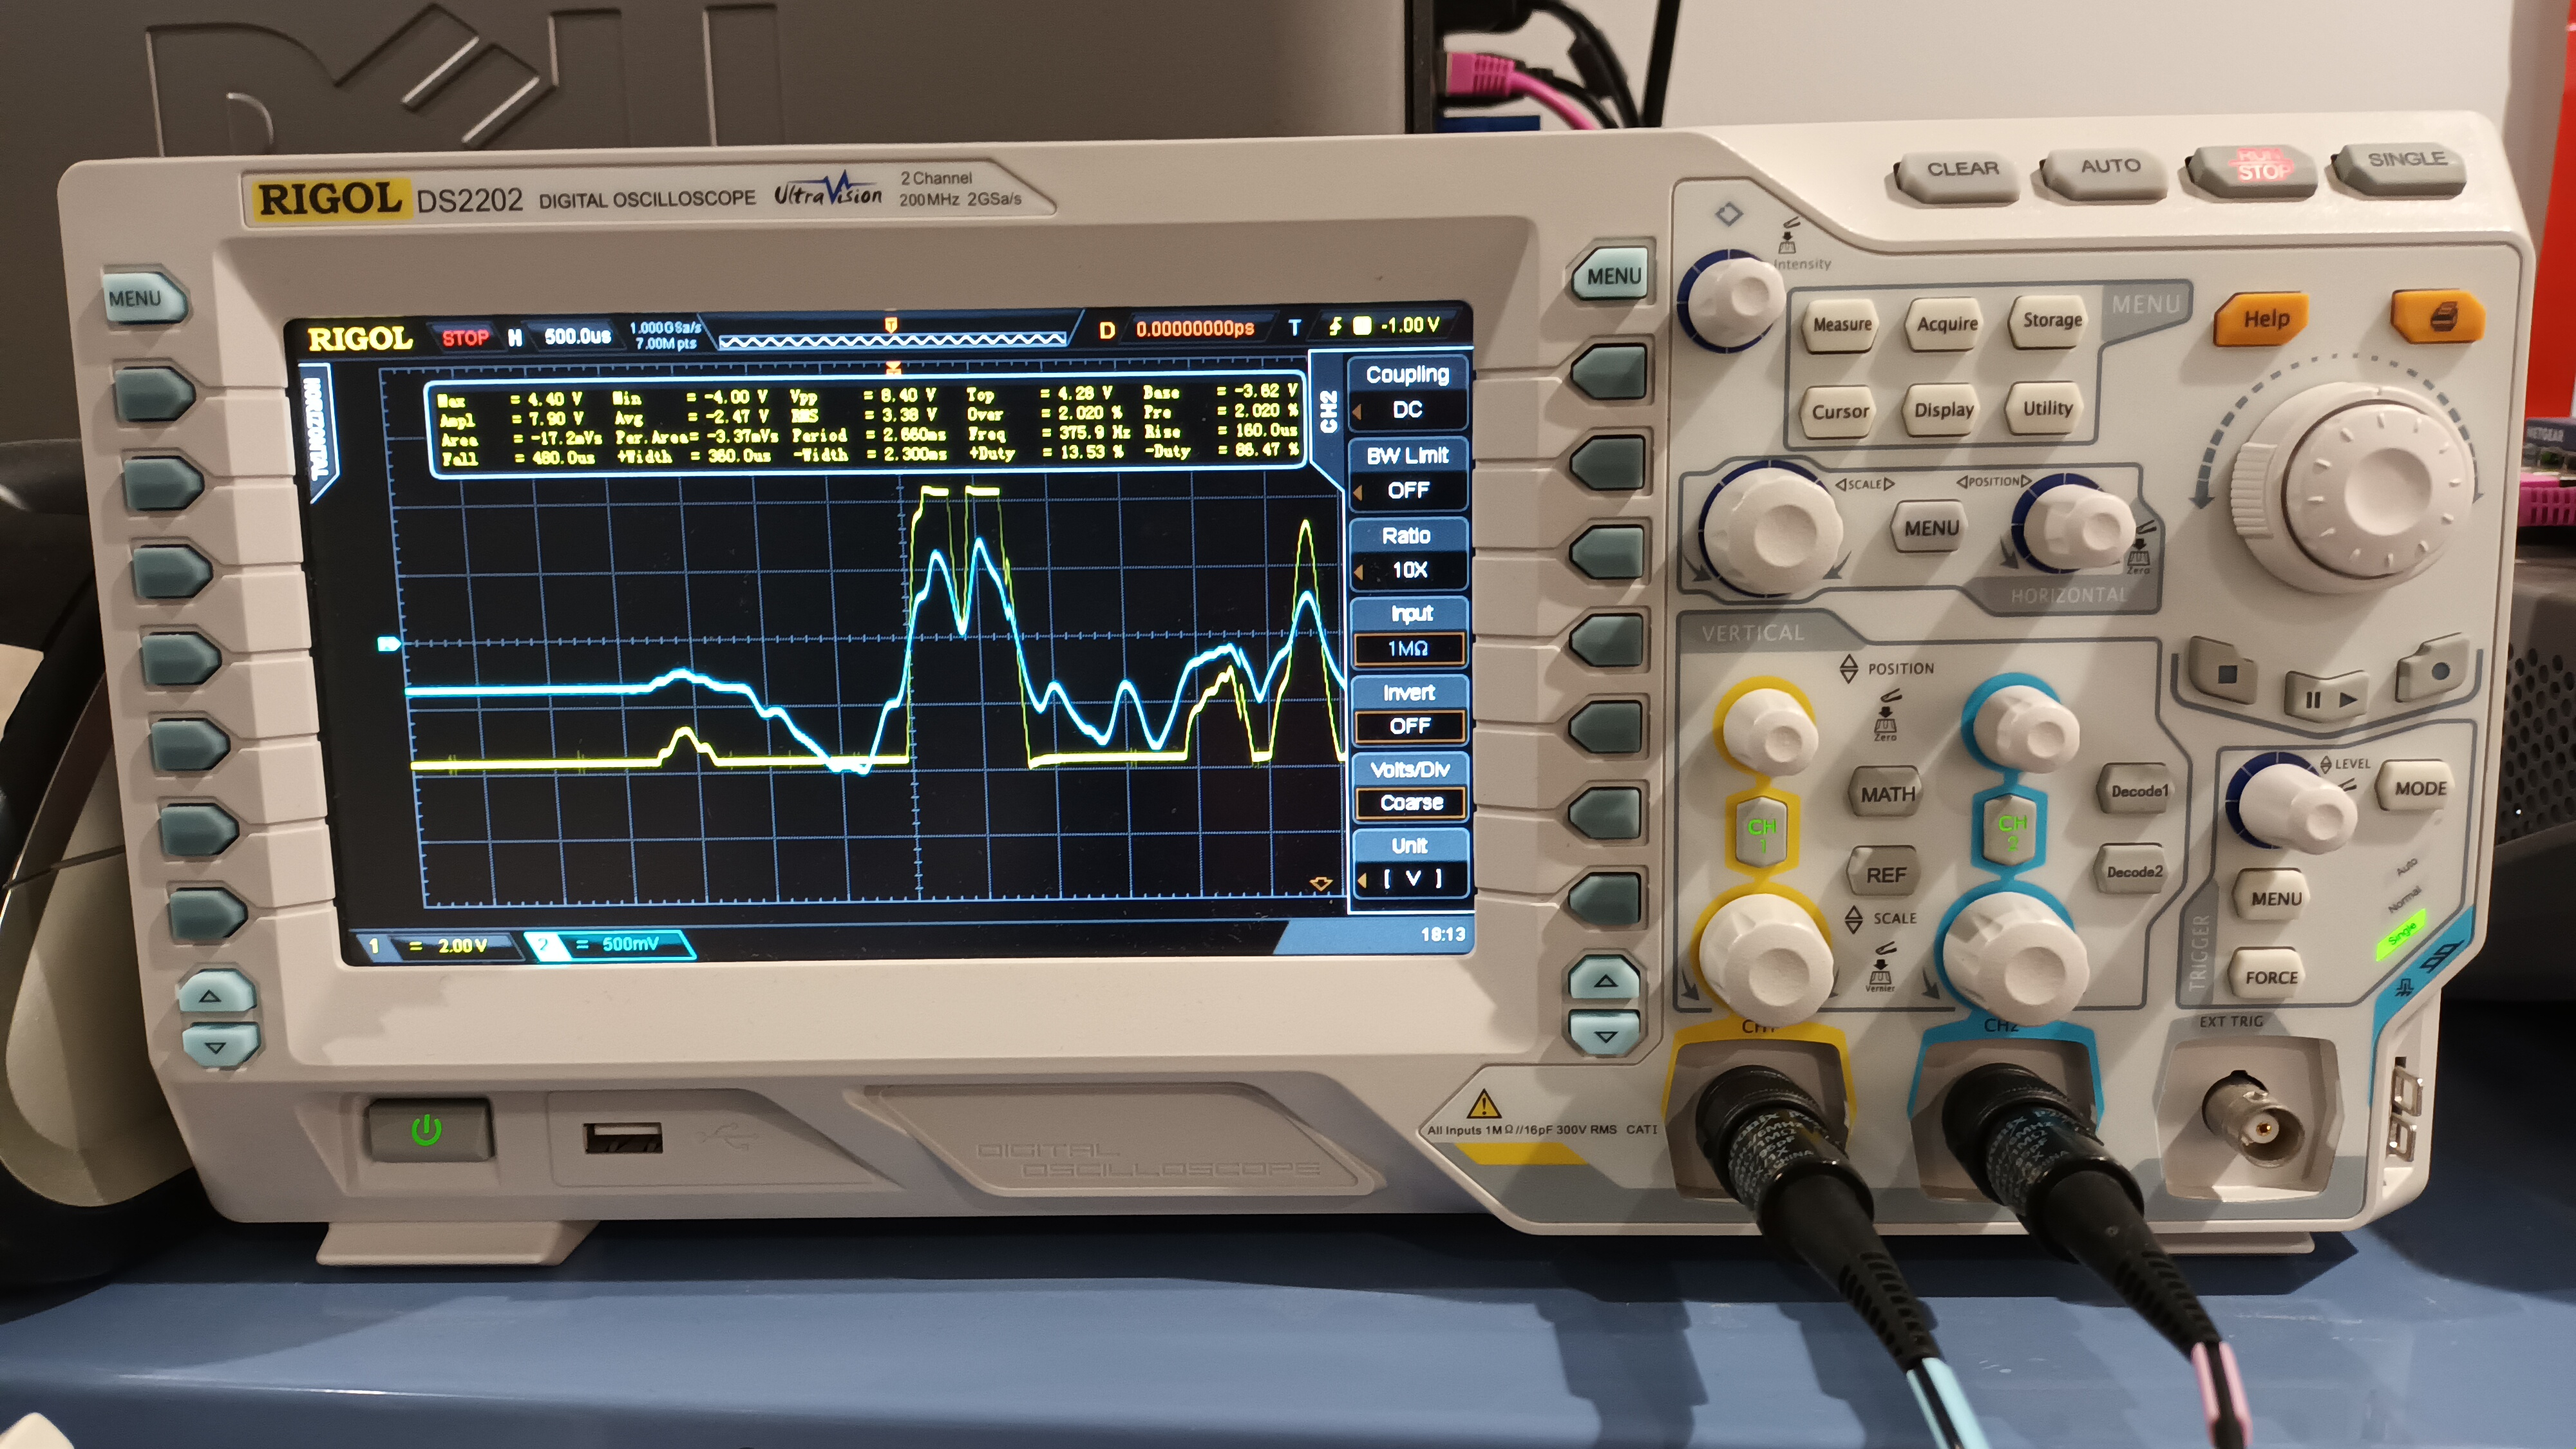
\includegraphics[scale=0.08]{sortie_osciloscope.jpg}
	\captionof{figure}{Comparatif post et pré-amplification}
	\label{image4}
\end{center}
\newpage
J'ai cependant rencontré plusieurs problèmes sur le montage de l'AOP. Tout d'abord n'étant pas habitué 
à les manipuler, j'ai confondu plusieurs fois les différentes broches de celui-ci. Ensuite, le souci majeur 
s'est trouvé au niveau de l'alimentation de celui-ci. L'alimentation par les broches V- et V+ devait se faire 
de manière symétrique. 
Âpres avoir solutionné tous ces problèmes, j'ai pu obtenir un premier montage fonctionnel.

\subsection{Liaisons des données}
L'arduino et le shield Ethernet sont fonctionnels et capables d'envoyer les données récoltées via MQTT.
\begin{center}	
	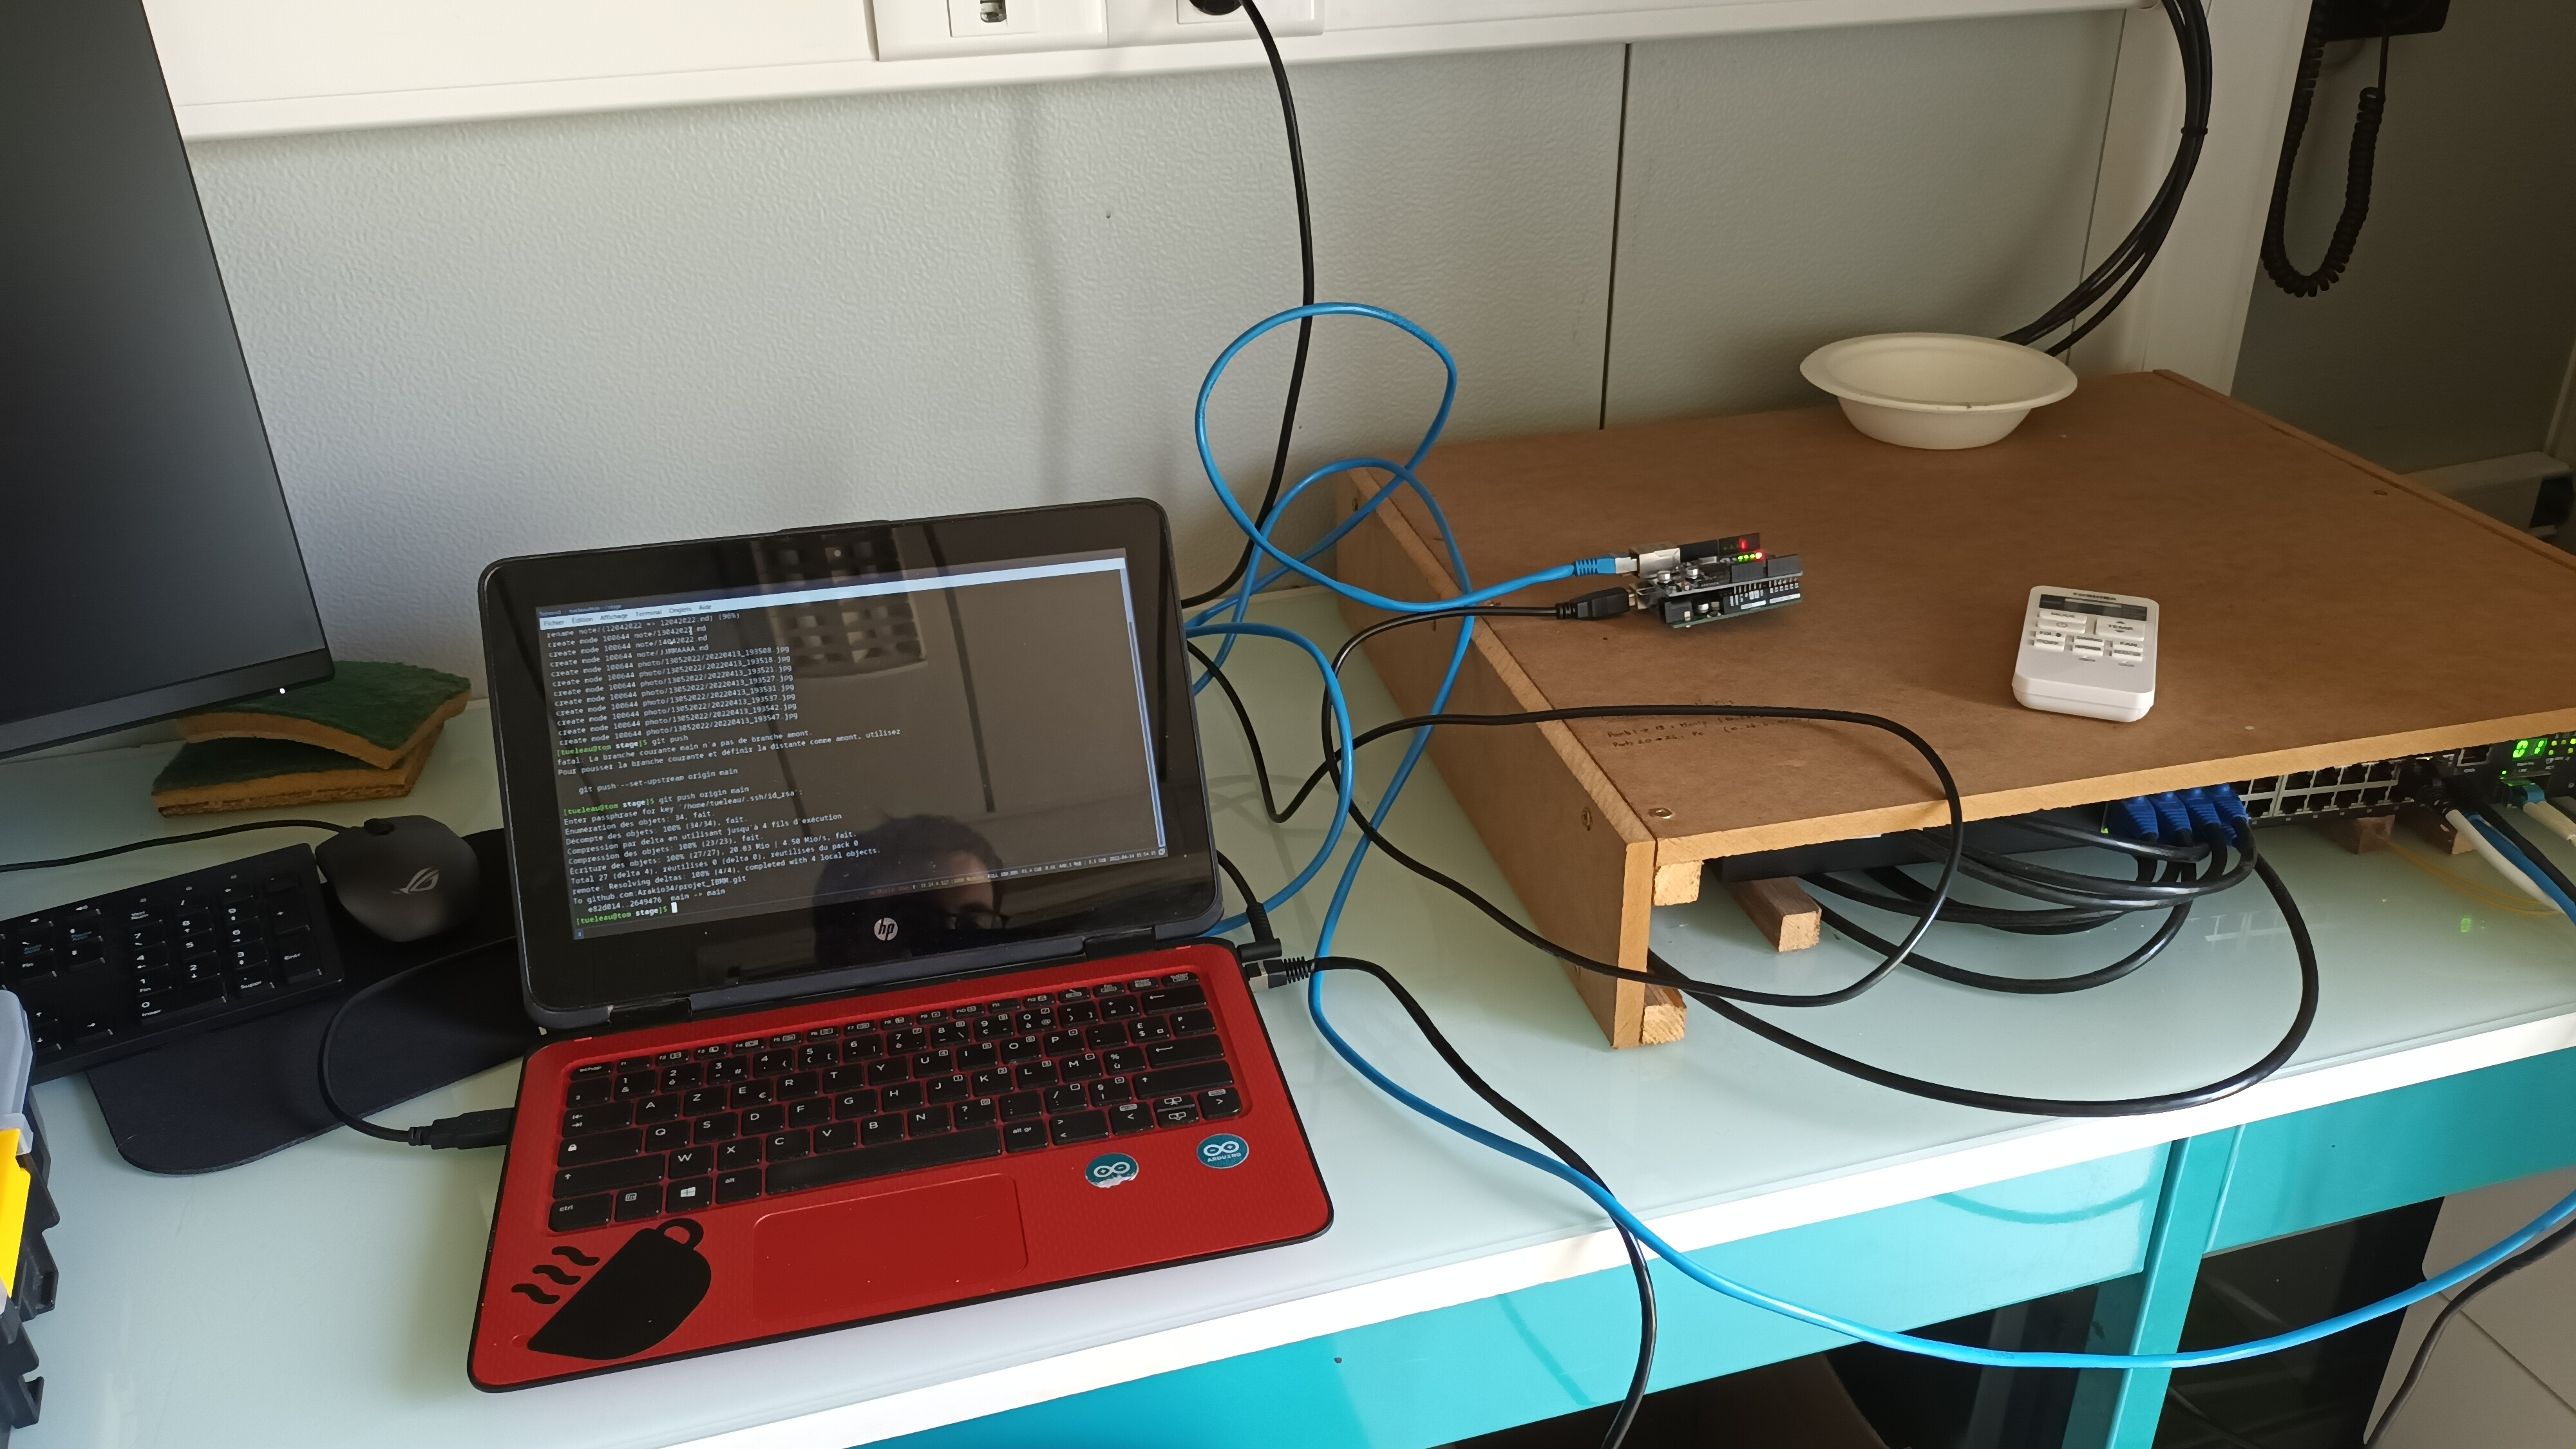
\includegraphics[scale=0.08]{shieldethernet.jpg}
	\captionof{figure}{Shield Ethernet}
	\label{image5}
\end{center}
\section{Travail à venir}
Mes objectifs pour la semaine à venir sont les suivants :\\
\\
	- Mieux comprendre les données récoltées par le capteur piezo\\
	- Débuter l'étude du micro\\
	- Terminer le montage AOP d'instrumentation\\
	- Mettre de premiers capteurs de température en fonctionnement\\
	- Étudier le travail de Kristine Branson\\

\newpage
\listoffigures
\end{document}
